%%%%%%%%%%%%%%%%%%%%%%%% editor.tex %%%%%%%%%%%%%%%%%%%%%%%%%%%%%
%
% root file for the contributions of a "contributed volume"
%
%%%%%%%%%%%%%%%%%%%%%%%%%%%%%%%%%%%%%%%%%%%%%%%%%%%%%%%%%%%%%%%%%

\documentclass[
graybox,
envcountchap,
tocaftauthskip,
12pt
]{svmult}

\usepackage{microtype}

%% use geometry to reduce the margins
\usepackage{geometry}
\geometry{
    letterpaper,
    heightrounded,
    hratio=1:1
}

%% set the reference style
\usepackage{nameref}
\usepackage[
natbib,
dashed=false,
defernumbers,
hyperref=true,
backend=biber,
uniquename=false,
style=authoryear-comp,
maxcitenames=2,
mincitenames=1,
maxbibnames=9,
uniquelist=false
]{biblatex}
\defbibheading{subbibliography}{%
    \section*{References for Section \ref{refsegment:\therefsegment}}}
\setlength\bibitemsep{5pt}
% Define external bib file
\addbibresource{zotero-refs-BLT.bib}


\usepackage{type1cm}        % activate if the above 3 fonts are 
                            % not available on your system
                             
\usepackage{comment}

\usepackage{makeidx}         % allows index generation
\usepackage{graphicx}        % standard LaTeX graphics tool
                             % when including figure files
% \usepackage{multicol}        % used for the two-column index
\usepackage[bottom]{footmisc}% places footnotes at page bottom

\usepackage{newtxtext}       % 
\usepackage{newtxmath}       % selects Times Roman as basic font

%\usepackage{mathptmx}       % selects Times Roman as basic font
\usepackage{helvet}          % selects Helvetica as sans-serif font

\usepackage{placeins}        % allows the use of floatbarriers
\usepackage{tabularx}        % creates tables that automatically adjust to contents
\usepackage{booktabs}        % allows the use of \midrule 
\usepackage{soul}            % highlighting
\usepackage{pdfpages}        % provide `\includepdf` command for inserting title page

\usepackage{threeparttable}

\usepackage{hyperref}
\usepackage{xcolor}
\hypersetup{
colorlinks,
linkcolor={red!50!black},
citecolor={blue!50!black},
urlcolor={blue!80!black}
}
%\hypersetup{colorlinks=false} % use true for debugging

% see the list of further useful packages in the Reference Guide

\makeindex             % used for the subject index
                       % please use the style svind.ist with
                       % your makeindex program

%%%%%%%%%%%%%%%%%%%%%%%%%%%%%%%%%%%%%%%%%%%%%%%%%%%%%%%%%%%%%%%%%

\usepackage{import}
% Define command `\segimport` to automatically create a 
% bibliography section for the imported file.
\newcommand{\seginclude}[1]{\endrefsegment\newrefsegment\include{#1}}
\newcommand{\segimport}[2]{\begin{refsegment}\import{#1}{#2}\end{refsegment}}

% include file with digital resource cite style

\providebool{bbx:subentry}
\newbibmacro*{citenum}{%Note: the original macro was called "cite". I did not redefine "cite", but instead defined a new macro "citenum", because the author-year citations use the "cite" macro too. "\renewbibmacro*{cite}" would have caused all the author-year citations to become numeric too.
  \printtext[bibhyperref]{%If you ever want to use hyperref
    \printfield{prefixnumber}%
    \printfield{labelnumber}%
    \ifbool{bbx:subentry}
      {\printfield{entrysetcount}}
      {}}}

\newbibmacro*{citetitle}{%
  \iffieldundef{shorthand}
  {\usebibmacro{cite:title}}%
  {\usebibmacro{cite:shorthand}}}

\newbibmacro*{cite:title}{%
  \printtext[bibhyperref]{%
    \printfield[citetitle]{labeltitle}}}

\DeclareCiteCommand{\citeprgm}
  {\usebibmacro{prenote}}
  {\usebibmacro{citeindex}%
   \usebibmacro{cite:title}%
   \printtext[bibhyperref]{ [\usebibmacro{citenum}]}%
   \usebibmacro{related:default}}%
  {\multicitedelim}
  {\usebibmacro{postnote}}


% Define checkmark symbol for appendix tables
\usepackage{tikz}
\def\checkmark{\tikz\fill[scale=0.4](0,.35) -- (.25,0) -- (1,.7) -- (.25,.15) -- cycle;}

\begin{document}

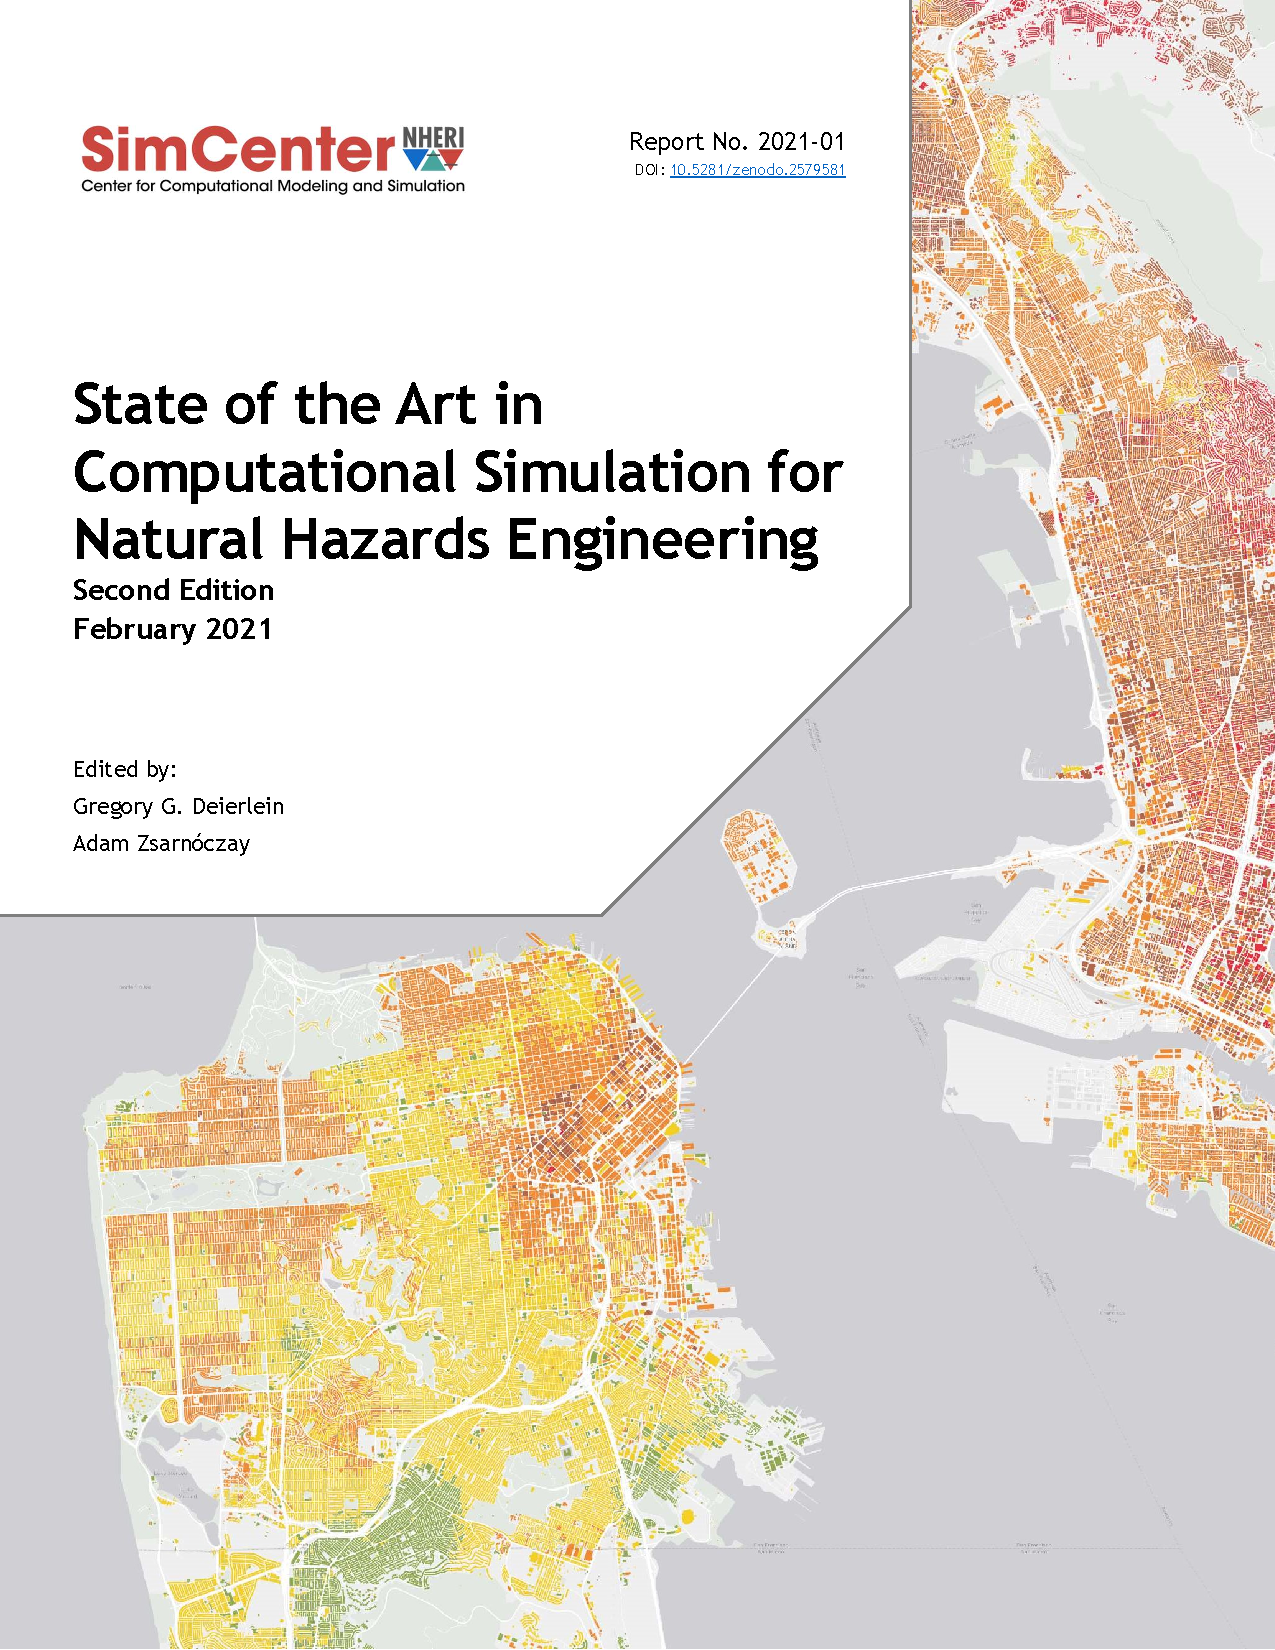
\includepdf[pages=-,fitpaper=true]{editor/cover_page.pdf}

\frontmatter%%%%%%%%%%%%%%%%%%%%%%%%%%%%%%%%%%%%%%%%%%%%%%%%%%%%%%

\import{editor/}{preface}
\import{editor/}{acknowledgement}

\setcounter{tocdepth}{1}

{\hypersetup{linkcolor=black}\tableofcontents}

\import{editor/}{contriblist}
\import{editor/}{acronym}

\mainmatter%%%%%%%%%%%%%%%%%%%%%%%%%%%%%%%%%%%%%%%%%%%%%%%%%%%%%%%

\segimport{editor/}{introduction}

\import{Hazard/}{main}
\segimport{Hazard/Earthquake_Ground_Shaking/}{main}
\segimport{Hazard/Earthquake_Surface_Rupture/}{main}
\segimport{Hazard/Earthquake_Liquefaction/}{main}
\segimport{Hazard/Earthquake_Landslide/}{main}
\segimport{Hazard/Storm_Wind/}{main}
\segimport{Hazard/Storm_Surge/}{main}
\segimport{Hazard/Tsunami/}{main}

\import{Response/}{main}
\segimport{Response/Structural/}{main}
\segimport{Response/Geotechnical/}{main}
\segimport{Response/CFD_Wind/}{main}
\segimport{Response/CFD_Water/}{main}

\import{Performance/}{main}
\segimport{Performance/Buildings/}{main}
\segimport{Performance/Transportation/}{main}
\segimport{Performance/Pipelines/}{main}
\segimport{Performance/Power/}{main}

\import{Recovery/}{main}
\segimport{Recovery/Communities/}{main}
\segimport{Recovery/Infrastructure_Systems/}{main}
\segimport{Recovery/Housing/}{main}
\segimport{Recovery/Businesses/}{main}

\import{CrossCutting/}{main}
\segimport{CrossCutting/Uncertainty/}{main}
\segimport{CrossCutting/AI/}{main}


\backmatter%%%%%%%%%%%%%%%%%%%%%%%%%%%%%%%%%%%%%%%%%%%%%%%%%%%%%%%

\begin{partbacktext}
\part{Appendix}
\appendix
\segimport{editor/}{appendix}
\end{partbacktext}

\part{References}\label{part:refs}

% \DeclareNameFormat{}{\usebibmacro{name:first-last}{}{#5}{#1}{#7}}

\Extrachap{Literature}

% \bibbysegment[heading=subbibliography,nottype=misc]
\printbibliography[segment= 1,nottype=software,title={Earthquake - Ground Shaking}]
\printbibliography[segment= 2,nottype=software,title={Earthquake - Ground Shaking}]
\printbibliography[segment= 3,nottype=software,title={Earthquake - Surface Fault Rupture}]
\printbibliography[segment= 4,nottype=software,title={Earthquake - Soil Liquefaction}]
\printbibliography[segment= 5,nottype=software,title={Earthquake - Slope Stability and Landslides}]
\printbibliography[segment= 6,nottype=software,title={Tropical Cyclone - Wind}]
\printbibliography[segment= 7,nottype=software,title={Tropical Cyclone - Storm Surge}]
\printbibliography[segment= 8,nottype=software,title={Tsunami - Inundation}]
\printbibliography[segment= 9,nottype=software,title={Structural Systems}]
\printbibliography[segment=10,nottype=software,title={Geotechnical Systems}]
\printbibliography[segment=11,nottype=software,title={Computational Fluid Dynamics - Wind}]
\printbibliography[segment=12,nottype=software,title={Computational Fluid Dynamics - Water}]
\printbibliography[segment=13,nottype=software,title={Buildings}]
\printbibliography[segment=14,nottype=software,title={Transportation Networks}]
\printbibliography[segment=15,nottype=software,title={Water, Sewer, and Gas Pipelines}]
\printbibliography[segment=16,nottype=software,title={Electrical Transmission Substations and Lines}]
\printbibliography[segment=17,nottype=software,title={Communities}]
\printbibliography[segment=18,nottype=software,title={Infrastructure Systems}]
\printbibliography[segment=19,nottype=software,title={Housing}]
\printbibliography[segment=20,nottype=software,title={Business}]
\printbibliography[segment=21,nottype=software,title={Uncertainty Quantification}]
\printbibliography[segment=22,nottype=software,title={Artificial Intelligence and Machine Learning}]
%---------------------------------------------
\defbibenvironment{bibliography}
{\list
{\printfield[labelnumberwidth]{labelnumber}}
{\setlength{\labelwidth}{\labelnumberwidth}%
\setlength{\leftmargin}{\labelwidth}%
\setlength{\labelsep}{\biblabelsep}%
\addtolength{\labelsep}{1em}
\addtolength{\leftmargin}{\labelsep}%
\setlength{\itemsep}{\bibitemsep}%
\setlength{\parsep}{\bibparsep}}%
\renewcommand*{\makelabel}[1]{\hss##1}}
{\endlist}
{\item}
\DeclareFieldFormat{labelnumberwidth}{\mkbibbrackets{#1}\hspace{-1.1em}}

\Extrachap{Digital Resources}

% \printbibliography[type=software,resetnumbers,title=Programs]
\printbibliography[segment= 1,resetnumbers,type=software,title={Introduction}]
\printbibliography[segment= 2,resetnumbers,type=software,title={Earthquake - Ground Shaking}]
\printbibliography[segment= 3,resetnumbers,type=software,title={Earthquake - Surface Fault Rupture}]
\printbibliography[segment= 4,resetnumbers,type=software,title={Earthquake - Soil Liquefaction}]
\printbibliography[segment= 5,type=software,title={Earthquake - Slope Stability and Landslides}]
\printbibliography[segment= 6,type=software,title={Tropical Cyclone - Wind}]
\printbibliography[segment= 7,type=software,title={Tropical Cyclone - Storm Surge}]
\printbibliography[segment= 8,type=software,title={Tsunami - Inundation}]
\printbibliography[segment= 9,type=software,title={Structural Systems}]
\printbibliography[segment=10,type=software,title={Geotechnical Systems}]
\printbibliography[segment=11,type=software,title={Computational Fluid Dynamics - Wind}]
\printbibliography[segment=12,type=software,title={Computational Fluid Dynamics - Water}]
\printbibliography[segment=13,type=software,title={Buildings}]
\printbibliography[segment=14,type=software,title={Transportation Networks}]
\printbibliography[segment=15,type=software,title={Water, Sewer, and Gas Pipelines}]
\printbibliography[segment=16,type=software,title={Electrical Transmission Substations and Lines}]
\printbibliography[segment=17,type=software,title={Communities}]
\printbibliography[segment=18,type=software,title={Infrastructure Systems}]
\printbibliography[segment=19,type=software,title={Housing}]
\printbibliography[segment=20,type=software,title={Business}]
\printbibliography[segment=21,type=software,title={Uncertainty Quantification}]
\printbibliography[segment=22,type=software,title={Artificial Intelligence and Machine Learning}]
%---------------------------------------------


%%%%%%%%%%%%%%%%%%%%%%%%%%%%%%%%%%%%%%%%%%%%%%%%%%%%%%%%%%%%%%%%%%%%%%




\printindex

%%%%%%%%%%%%%%%%%%%%%%%%%%%%%%%%%%%%%%%%%%%%%%%%%%%%%%%%%%%%%%%%%%%%%%

\end{document}

